\chapter{Introduction}
\section{The Large Hadron Collider}
The Large Hadron Collider is the most powerful particle accelerator in the world, located in CERN on the France-Swiss border.
The circumference of the LHC is 27km, and is located 100m underground. 
The maximum energy possible to accelerate the particles to in the LHC is directly dependent on the size of the LHC and the strength of the magnets used to accelerate the particles. 
In order to achieve the design energy of 7 TeV per proton, it was necessary to have a circumference of 27km, and to use some of the most powerful dipoles and radiofrequency cavities in existence. 
Inside the pipes where the protons travel, a very strong vacuum is required, and so the pressure in some parts is over $10^{-9}Pa$. 
The beams are made up of cylinder-like bunches. 
Using these bunches, the expected number of collisions is $10^{34}$ per $cm^2$ per second. If we take into account the cross section of the proton-proton interaction, roughly $100$mBarns ($1\textrm{Barn}=10^{-24}\textrm{cm}^{2}$), then the expected number of proton proton interactions is:
\begin{align}
10^{34}\textrm{cm}^{-2}\textrm{s}^{-1}(100\textrm{mBarns})\frac{1 \textrm{Barn}}{1000\textrm{mBarn}}\frac{10^{-24}\textrm{cm}^2}{1\textrm{Barn}}=10^{9}\textrm{s}^{-1}
		\label{proton-proton collisions per second}
\end{align}
The time between bunches is about $25ns$, so in theory, there could be about $3550$ bunches in the entire circumference of the LHC, but in practice there are only usually a maximum of 2556 bunches in either direction when the LHC is filled.
\section{ATLAS Experiment}
\textbf{ATLAS (A Toroidal LHC ApparatuS)} is one of seven particle detector experiments constructed at the Large Hadron Collider, a particle accelerator at CERN. 
When the LHC runs at full energy and intensity, there are bunch crossings every 25 nanoseconds, which mean there are about 25 million proton-proton collisions taking place every second inside the ATLAS detector. 
The amount of data collected for each event is around 1MB. For the ATLAS experiment, there is about a gigabyte of data collected each second. 
Because this is significantly larger than any practical system can handle, there are \textbf{triggers} that are designed to reject uninteresting events and keep the interesting ones. 
For ATLAS, the trigger system is designed to run at about 1kHz or 1000 events per second. 
This means that ATLAS collects about 4 petabytes of data per year. 
There are $10^{11}$ protons in a bunch. 
The proton-proton interaction cross section is approximately $100mB$.
\section{Trigger System}
In particle physics, a trigger is a system that uses simple criteria to rapidly decide which events in a particle detector to keep when only a small fraction of the total can be recorded.
The trigger system is necessary because of limitations in terms of data storage capacity and rates. 
In general, the experiments typically search for ``interesting'' events (decays of rare particles) that occur at relatively low rates, so we need to have trigger systems that identify events that should be recorded for later analysis. 
The Large Hadron Collider has an event rate of approximately 1 GHz. 
The triggers are divided into levels so that each level selects the data that becomes an input for the next level, which has more time available and more information to make better decisions.
There is the \textbf{Level-1 (L1)} system, which is based on custom electronics, and the \textbf{High Level Trigger (HLT)} system, that relies on commercial processors. 
The L1 system uses only coarsely segmented data from the calorimeter and muon detectors, while holding all the high-resolution data in pipeline memories in the electronics.
\section{Missing Transverse Momentum}
The transverse momentum is defined to be the momentum in the transverse plane to the beam axis. 
Because the protons in the beam pipe collide approximately head-on in opposite directions, we expect the produced particles to have approximately zero momentum. 
As a result, we know we must conserve transverse momentum. Longitudinal momentum is also conserved, but because it is very difficult to measure the momentum in the direction of the axis of the beam pipe, the detector is not able to measure it. 
The total transverse momentum is defined to be the vector sum of the transverse momenta of the particles produced in the beam pipe. 
When the vector sum of the transverse momenta of the particles produced is not zero, we say there is some ``missing'' transverse momentum. 
There are sources of missing transverse momentum that are due to noise in the detector, and then there are sources of missing transverse momentum that are due to real particles escaping the detector. 
One particle that escapes the detector without being detected is the neutrino. Because the neutrino has zero net charge and interacts only weakly, it is a prime source of real missing transverse momentum. 
Because we know one of the decay processes for producing a neutrino is the W boson decaying into a muon and a neutrino, we can calibrate the efficiency of our algorithms for selecting events with real missing transverse momentum by only considering events with a transverse mass similar to that of the W boson, and where the muon trigger fired (meaning a muon was detected)
\section{Efficiency Curves}
An efficiency curve illustrates the probability of an algorithm to classify the MET of an event as above or below a threshold value as a function of the MET as determined by another, ``true'' algorithm. 
So we can ask, what is the efficiency of L1 $> 30$ as a function of CELL MET. What this is means is we are taking the MET as determined by CELL to be the true MET, and we want to know how well (what the probability is) L1 does at classifying events as having MET above or below $30$ at each value of the MET determined by CELL. 
The way one would read a plot of this efficiency is to pick a value of CELL MET ( on the x-axis ) and ask ``of the number of events CELL determined had this MET, what fraction did L1 determine had MET greater than the threshold [30 GeV]''. 
The fraction [of the total amount of events CELL determined was in that MET bin] that L1 determined was greater than the threshold would be the height of the efficiency curve at that value of CELL MET.
A perfect efficiency curve would look like a step function centered at the threshold around which one is trying to classify the MET of events. Consider figure \ref{perfEff}. This is a plot of the efficiency of $L1>60 GeV$ as a function of L1 MET. It is a step function because if you take a point on the x axis lower than the threshold, you would expect there to be no events L1 said was greater than the threshold, thus yielding a zero efficiency. The same reasoning holds for points to the right of the threshold.
The fact that efficiency curves in reality do not look like step functions can be understood in terms of Type I and Type II error. 
The step function for the efficiency curve would be centered on the threshold one is asking for the efficiency about. Consider figure \ref{imperfEff}. This is a plot of the efficiency of $L1>60 GeV$, as a function of CELL MET.
The fact that the efficiency curve immediately to the left of the threshold is not zero means that, of the events CELL determined had MET lower than the threshold, L1 determined some fraction of those events had an MET higher than the threshold. 
The fact that the efficiency curve immediately to the right of the threshold is not one means that, of the events CELL said had MET larger than the threshold, L1 said some fraction of those events had MET lower than the threshold. 
In this case, the fraction of events L1 determined had an MET higher than the threshold, given that CELL said the MET was higher than the threshold, is less than one.
\pagebreak
\begin{figure}[h]
        \centering
        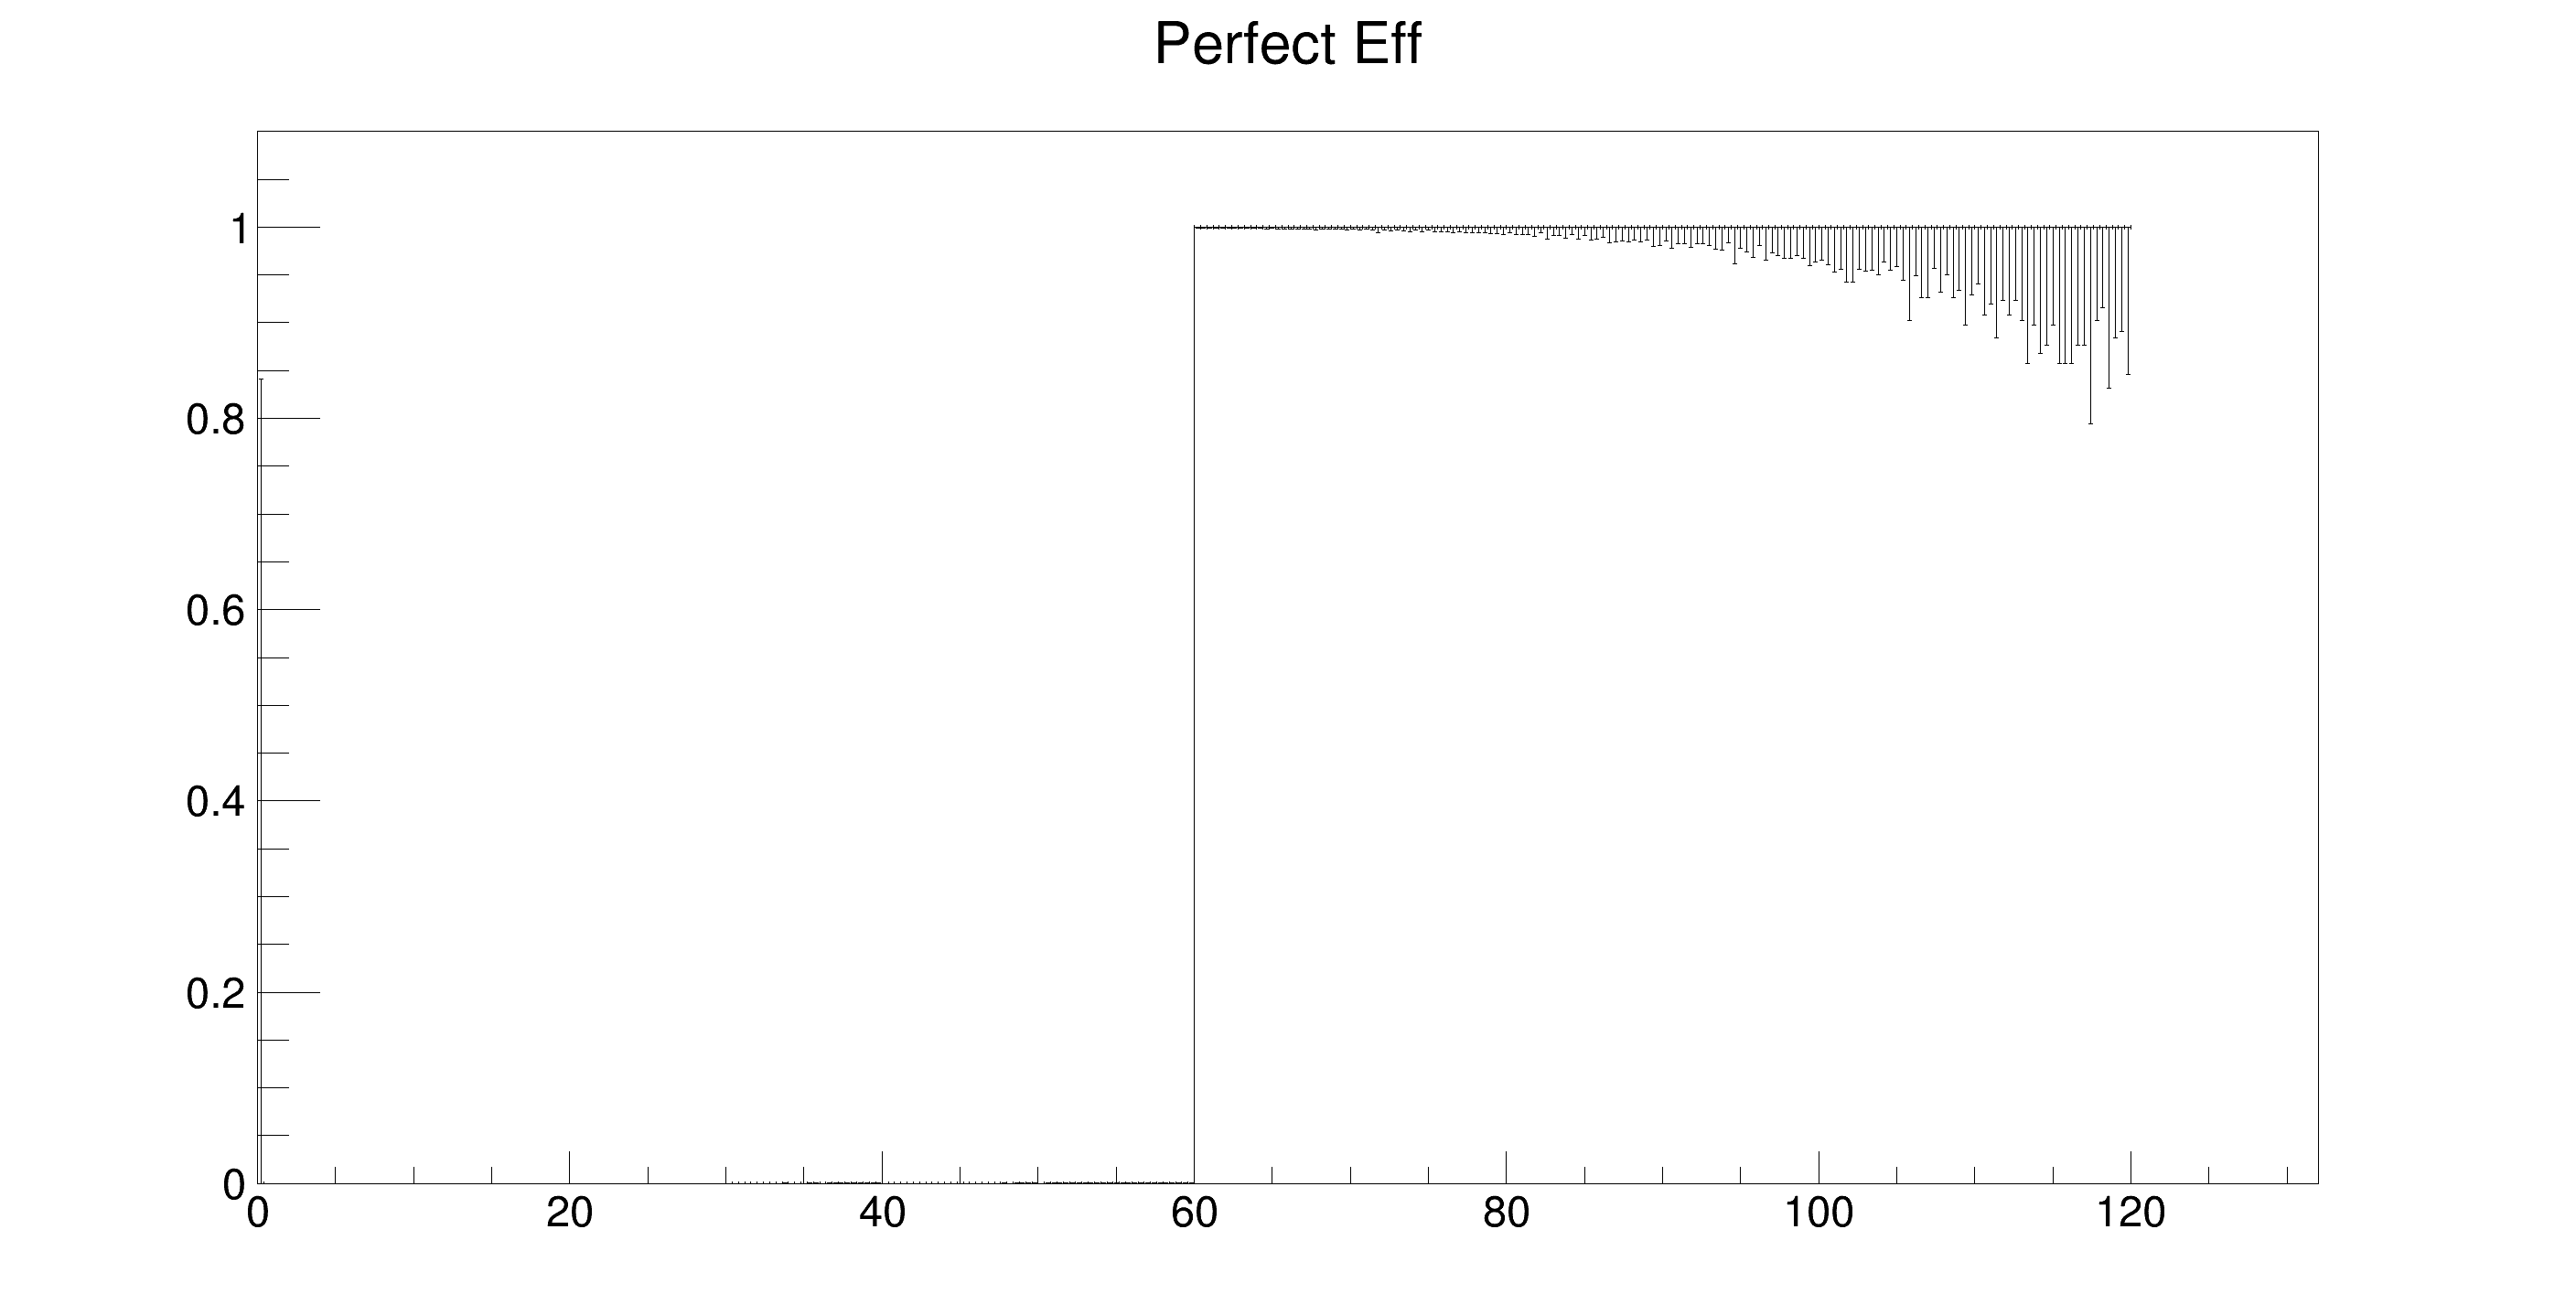
\includegraphics[scale=0.125]{perfectEfficiency}
        \caption{An example of a perfect efficiency curve for $\textrm{L1}>60\textrm{GeV}$}
        \label{perfEff}
\end{figure}
\begin{figure}[h]
        \centering
        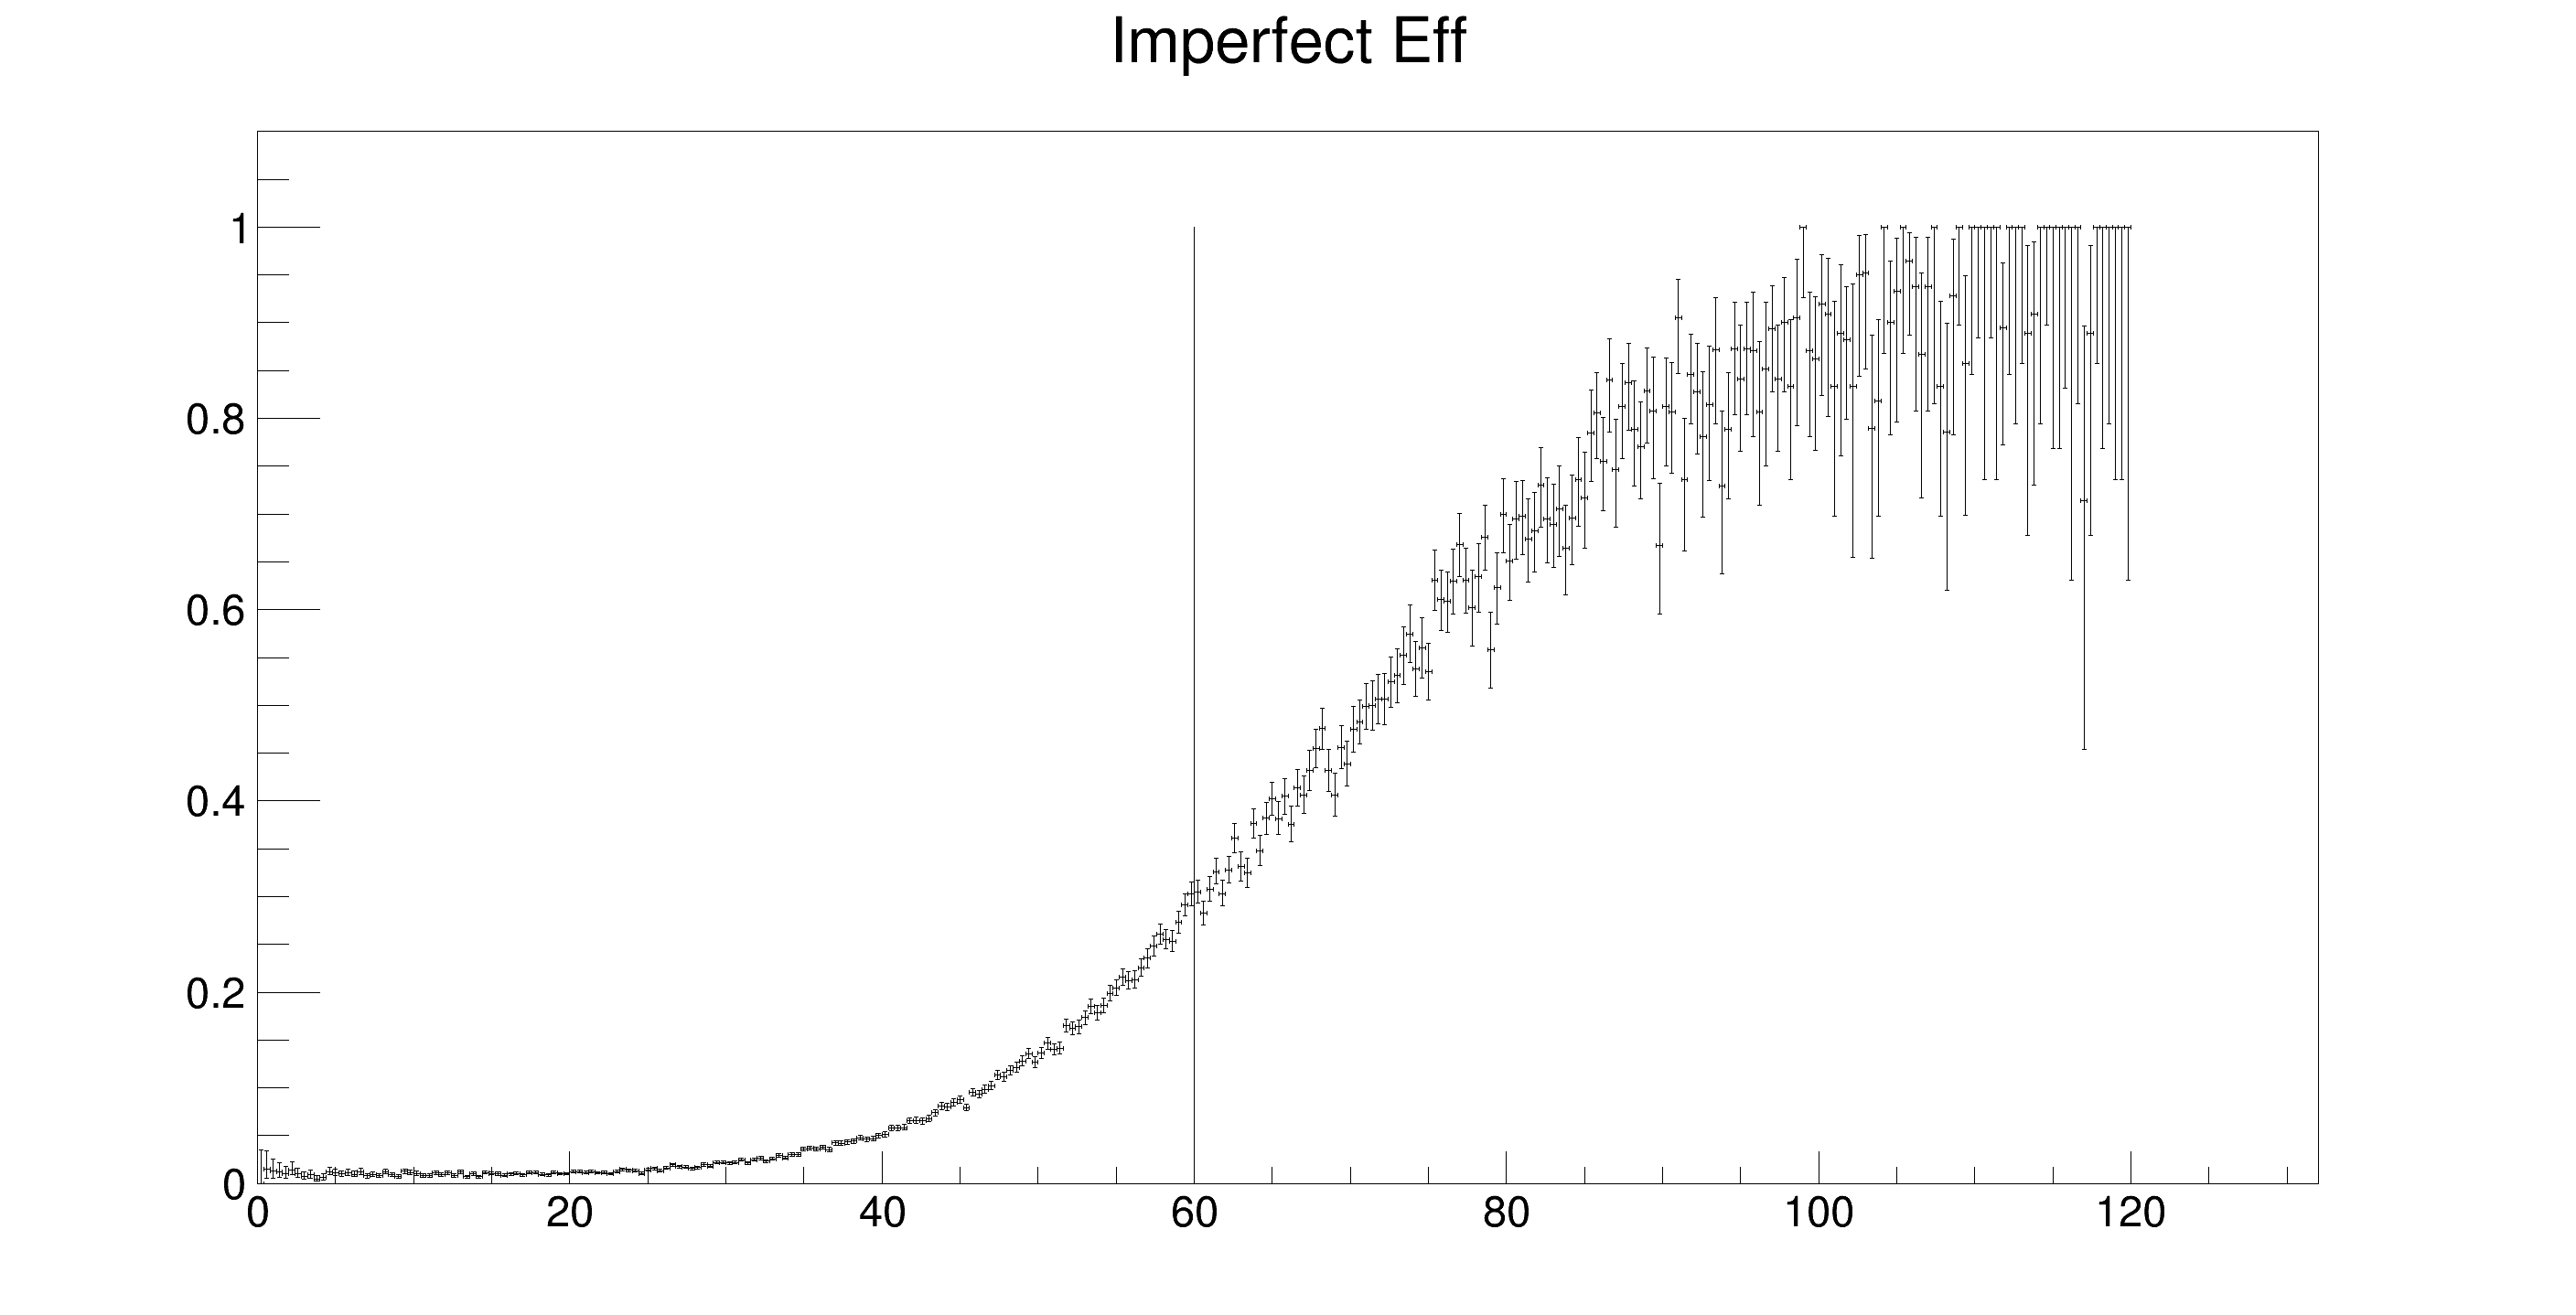
\includegraphics[scale=0.125]{imperfectEfficiency}
        \caption{An example of an imperfect efficiency curve for $\textrm{L1}>60\textrm{GeV}$}
        \label{imperfEff}
\end{figure}
